\section{3D Geometry}
\label{sec:3d_geometry}

\begin{frame}
    \frametitle{3D coordinates}
    \begin{figure}
        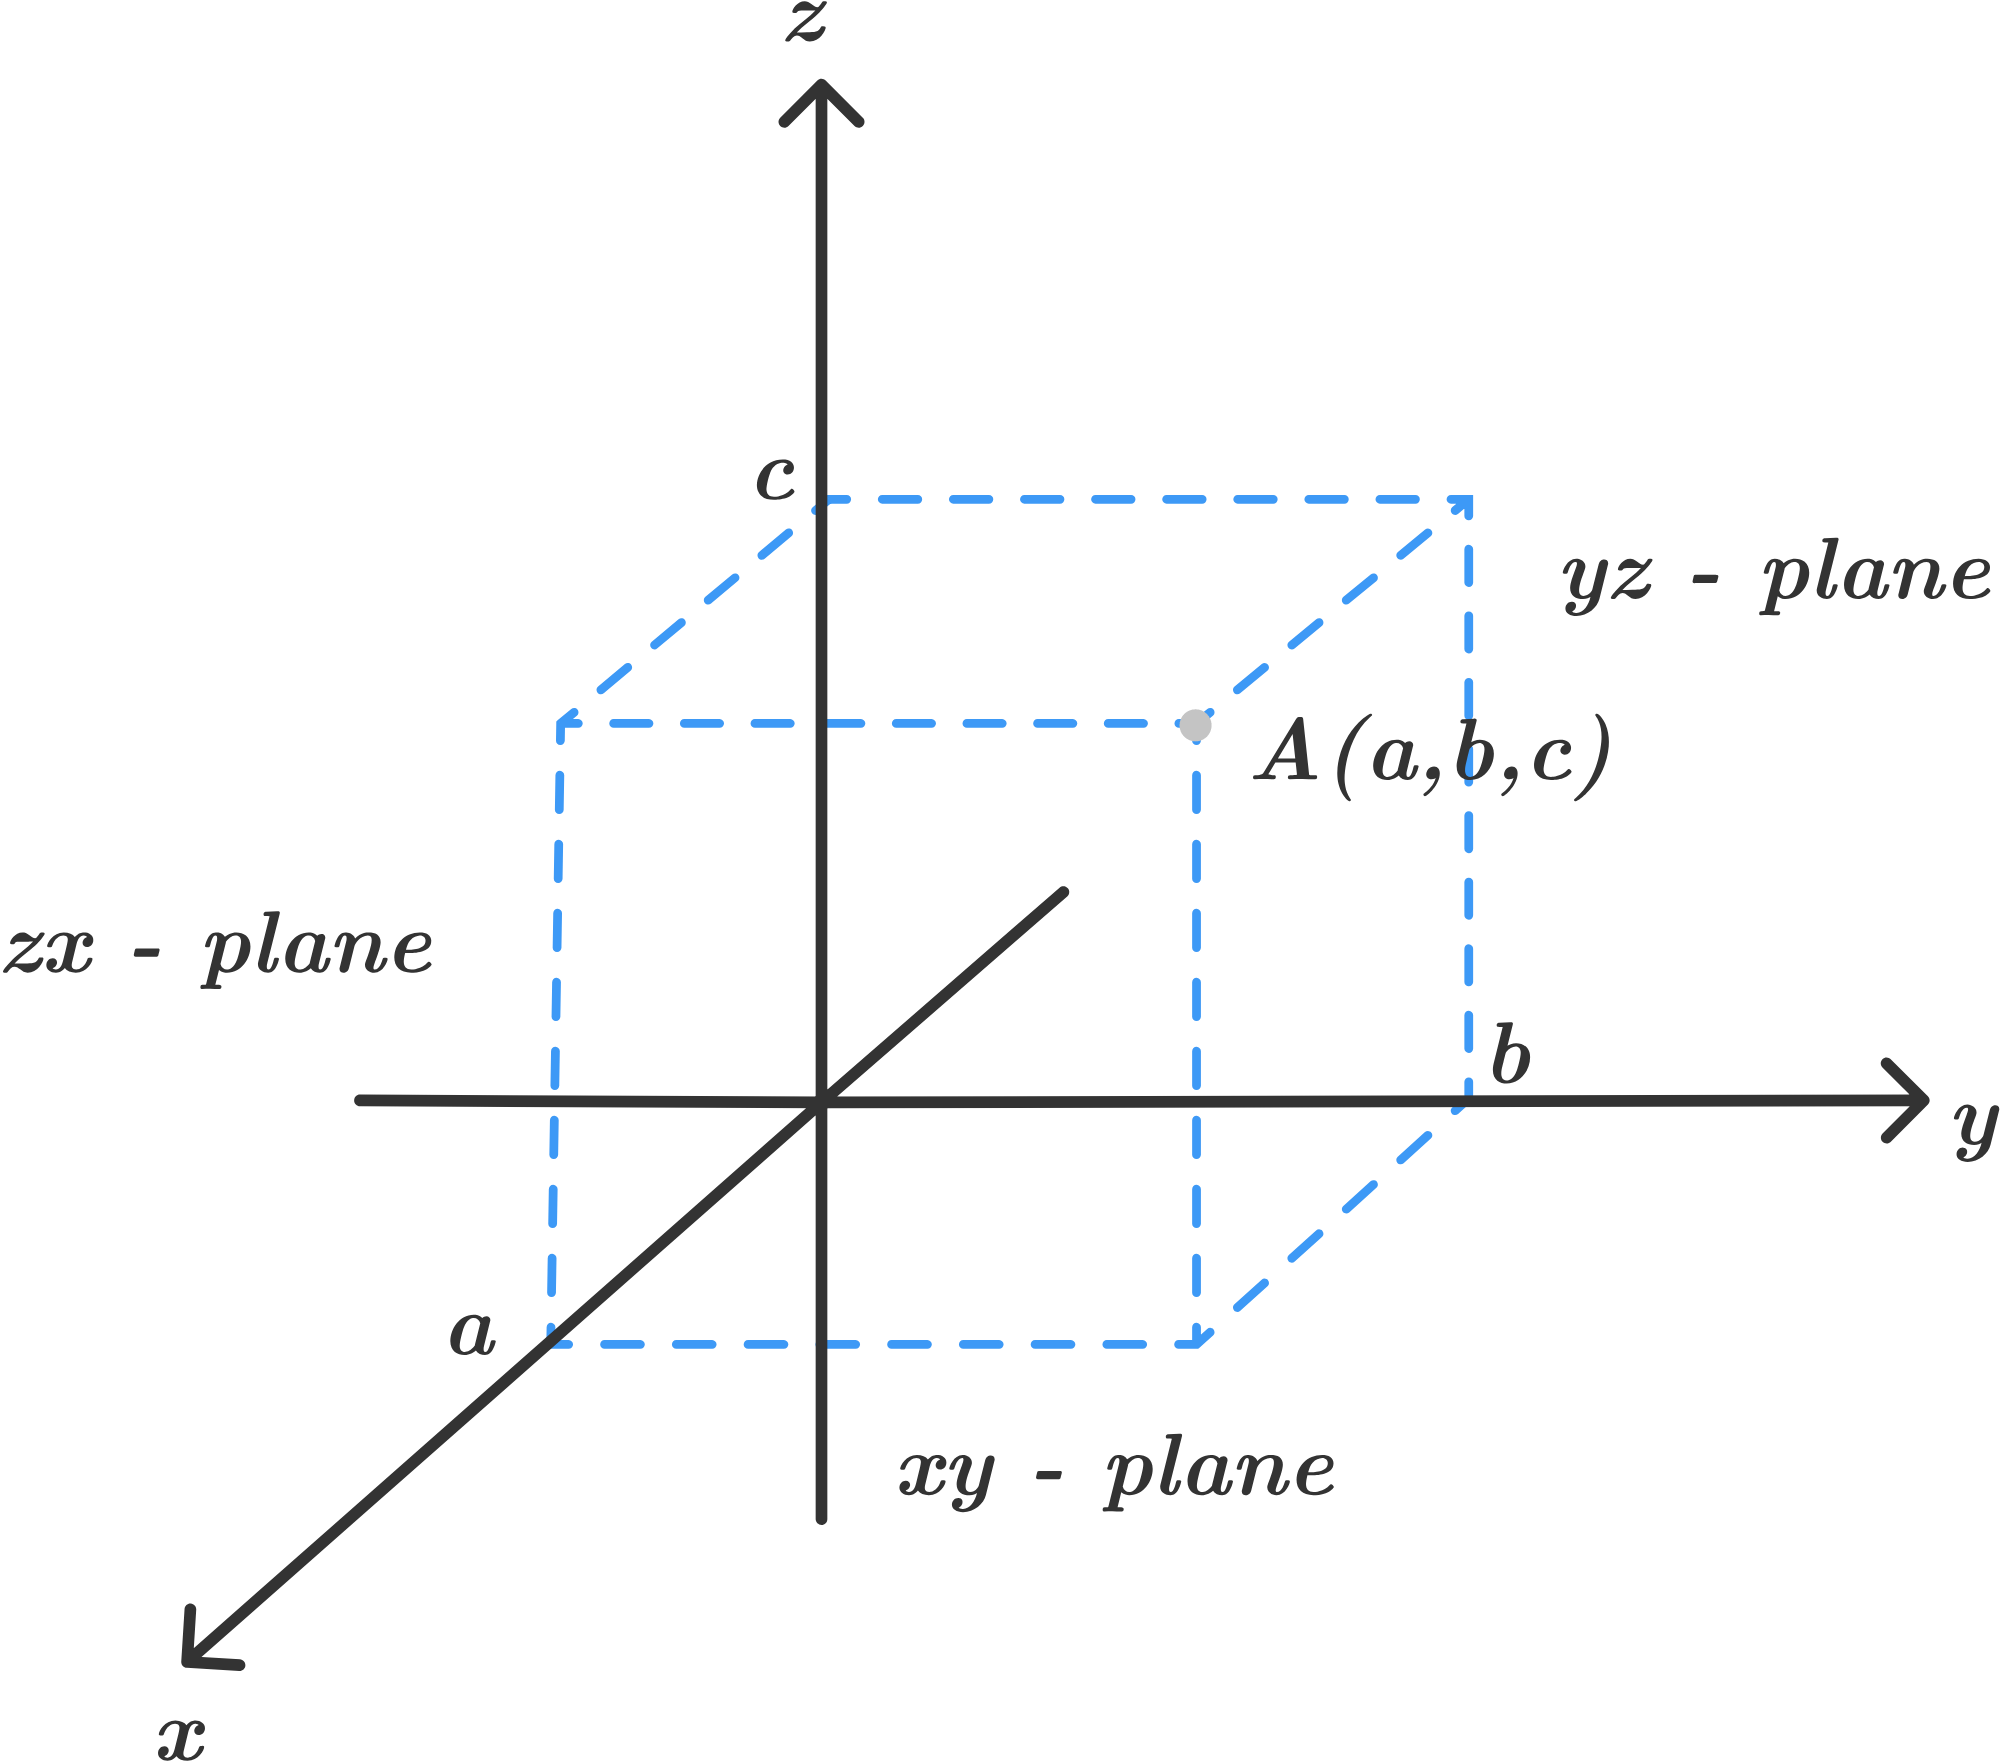
\includegraphics[scale=0.1]{3d_geometry/co_ordinate_plane.png}
        \caption{3D Coordinate Plane}
    \end{figure}
\end{frame}

\begin{frame}
    \frametitle{3D Coordinate System}
    \begin{itemize}
        \item The 3D coordinate system is defined by three mutually perpendicular axes: the x-axis, y-axis, and z-axis.
        \item A point in 3D space is represented by its coordinates \(P(x, y, z)\).
        \item The position vector of a point \(P\) in 3D space is given by:
        \[
        \vec{OP} = x\hat{\imath} + y\hat{\jmath} + z\hat{k}
        \]
    \end{itemize}       
\end{frame}

\begin{frame}
    \frametitle{Shifting the Origin}
    \begin{block}{Translation of Axes}
        Shifting the origin  to another point without changing the direction of axes is called \textbf{translation}.
    \end{block}
   Let the origin \(O\) be shifted to a new point \(O'\) with coordinates \(O'(x_0, y_0, z_0)\). The position vector of a point \(P(x,y,z)\) with respect to the new origin \(O'\) given by :
    \[
        \vec{O'P} = (x - x_0)\hat{\imath} + (y - y_0)\hat{\jmath} + (z - z_0)\hat{k}
    \]
\end{frame}

\begin{frame}
\frametitle{Distance Formula in 3D}
\begin{figure}
    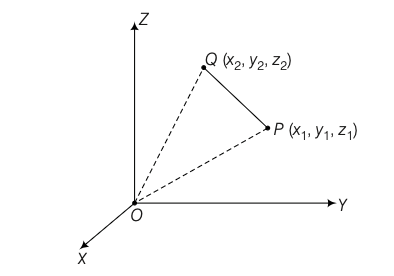
\includegraphics[scale=0.1]{3d_geometry/distance.png}
    \caption{Distance Formula in 3D}
\end{figure}
Let \(OP = x \hat{\imath} + y \hat{\jmath} + z \hat{k}\)  and \(OQ = x' \hat{\imath} + y' \hat{\jmath} + z' \hat{k}\) be two points in 3D space. The distance \(d\) between points \(P\) and \(Q\) is given by the formula:
\begin{align*}
    \vec{OQ} &= \vec{OP} + \vec{PQ} \\
    \vec{PQ} &= \vec{OQ} - \vec{OP} \\
    d &= |\vec{PQ}| = \sqrt{(x' - x)^2 + (y' - y)^2 + (z' - z)^2}
\end{align*}
\end{frame}

\begin{frame}
    \frametitle{Section Formula}
    \begin{figure}
        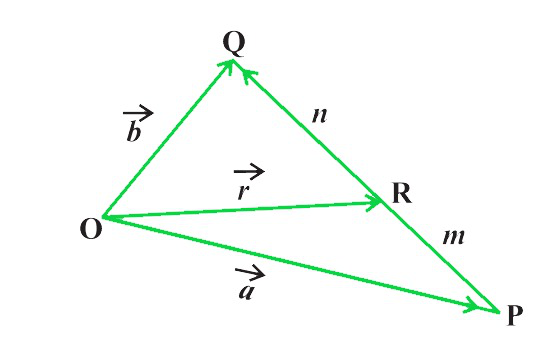
\includegraphics[scale=0.3]{3d_geometry/section.png}
        \caption{Section Formula in 2D}
    \end{figure} 
\end{frame}


\begin{frame}
    \begin{block}{Section Formula in 3D}
    Let \(P(x_1, y_1, z_1)\) and \(Q(x_2, y_2, z_2)\) be two points in 3D space with position vectors \( \vec{\mathbf{r}_1} \), \( \vec{\mathbf{r}_2} \) respectively. If a point \(R\) divides the line segment \(PQ\) in the ratio \(m:n\), then the position vector of point \(R\) is given by:
    \[
    \vec{\mathbf{r}} = \frac{m\vec{\mathbf{r}_2} + n\vec{\mathbf{r}_1}}{m+n}
    \]
    \end{block}
\end{frame}

\begin{frame}
    \frametitle{Proof of Section Formula}
    \begin{block}{Given}
    Point \(R\) divides line segment \(PQ\) internally in the ratio \(m:n\), where \(P\) and \(Q\) have position vectors \(\vec{\mathbf{a}}\) and \(\vec{\mathbf{b}}\) respectively.
    \end{block}
    
    \begin{block}{To Prove}
    The position vector of \(R\) is \(\vec{\mathbf{r}} = \frac{m\vec{\mathbf{b}} + n\vec{\mathbf{a}}}{m+n}\)
    \end{block}
    
    \begin{block}{Proof}
    Since \(R\) divides \(PQ\) in ratio \(m:n\):
    \begin{align}
        \frac{|\vec{PR}|}{|\vec{RQ}|} &= \frac{m}{n} \\
        \text{Since } \vec{PR} \text{ and } \vec{RQ} \text{ are collinear:} \quad \vec{PR} &= \frac{m}{n}\vec{RQ}
    \end{align}
    \end{block}
\end{frame}

\begin{frame}
    \frametitle{Proof of Section Formula (continued)}
    
    From vector addition: \(\vec{PR} + \vec{RQ} = \vec{PQ}\)
    
    Substituting \(\vec{PR} = \frac{m}{n}\vec{RQ}\):
    \begin{align}
        \frac{m}{n}\vec{RQ} + \vec{RQ} &= \vec{PQ} \\
        \vec{RQ}\left(\frac{m}{n} + 1\right) &= \vec{PQ} \\
        \vec{RQ} &= \frac{n}{m+n}\vec{PQ}
    \end{align}

\end{frame}


\begin{frame}
 
    Since \(\vec{PQ} = \vec{\mathbf{b}} - \vec{\mathbf{a}}\) and \(\vec{RQ} = \vec{\mathbf{b}} - \vec{\mathbf{r}}\):
    \begin{align}
        \vec{\mathbf{b}} - \vec{\mathbf{r}} &= \frac{n}{m+n}(\vec{\mathbf{b}} - \vec{\mathbf{a}}) \\
        \vec{\mathbf{r}} &= \vec{\mathbf{b}} - \frac{n}{m+n}(\vec{\mathbf{b}} - \vec{\mathbf{a}}) \\
        \vec{\mathbf{r}} &= \frac{m\vec{\mathbf{b}} + n\vec{\mathbf{a}}}{m+n}
    \end{align}
  
\end{frame}

\begin{frame}
\frametitle{Direction Ratios}
\begin{block}{Direction Ratios}
    The direction ratios of a line are any three numbers that are proportional to the direction cosines of the line. If a line has direction cosines \(l, m, n\), then its direction ratios can be represented as \(a, b, c\) such that:
    \begin{align*}
        l = \frac{a}{\sqrt{a^2 + b^2 + c^2}}, \quad m = \frac{b}{\sqrt{a^2 + b^2 + c^2}}, \quad n = \frac{c}{\sqrt{a^2 + b^2 + c^2}} 
        l &= k a \\
        m &= k b \\
        n &= k c
    \end{align*}
\end{block} 
\begin{itemize}
    \item It is evident that the direction ratios are not unique, as they can be scaled by any non-zero constant \(k\).
    \item However, the ratios \(a:b:c\) remain constant regardless of the scaling
\end{itemize}
\end{frame}

\begin{frame}
    \frametitle{Equation of a Line passing through a given point and parallel to a given vector}
    \begin{figure}
        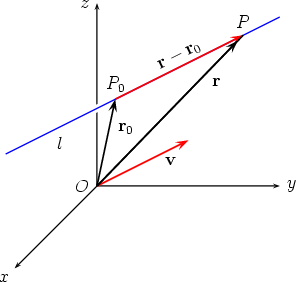
\includegraphics[scale=0.4]{3d_geometry/line_parallel_vector.png}
        \caption{Line in 3D space}
    \end{figure}
\end{frame}


\begin{frame}
\frametitle{Equation of a Line passing through a given point and parallel to a given vector}
    Let \(P_{0}(x_0, y_0, z_0)\) be a point on the line and \(P_{1}(x_1, y_1, z_1)\) be another point on the line. The direction vector of the line can be defined as \(\vec{P_{0}P_{1}} = \vec{r}_1 - \vec{r}_0\), where \(\vec{r}_0\) and \(\vec{r}_1\) are the position vectors of \(P_0\) and \(P_1\) respectively. The vector equation of the line can be expressed as:
    \[
    \vec{r} - \vec{r_0} = t\vec{v}
    \]
    where \(t\) is a scalar parameter. 
\end{frame}

\begin{frame}
    \frametitle{Direction Cosines vs. Direction Ratios: The Intuition}
    \begin{itemize}
        \item \textbf{Direction Cosines (DCs):} A unique, standardized recipe. They tell you how much to travel along each axis to move exactly one unit along the line. The sum of their squares is always 1: \(l^2 + m^2 + n^2 = 1\).
        \item \textbf{Direction Ratios (DRs):} A flexible, proportional recipe. They tell you the ratio of movement along the axes. For every 'a' units in x, you move 'b' units in y and 'c' units in z. They are not unique; any scalar multiple represents the same direction.
    \end{itemize}
\end{frame}

\begin{frame}
    \frametitle{Direction Cosines (DCs): Mathematical Definition}
    Let a vector \(\vec{v}\) make angles \(\alpha, \beta, \gamma\) with the positive X, Y, and Z axes.
    \begin{itemize}
        \item \(l = \cos(\alpha)\)
        \item \(m = \cos(\beta)\)
        \item \(n = \cos(\gamma)\)
    \end{itemize}
    \begin{figure}
        \includegraphics[width=0.6\textwidth]{direction_cosine_angles.png}
        \caption{Angles for Direction Cosines}
    \end{figure}
    For a vector \(\vec{v} = (x, y, z)\) with magnitude \(|\vec{v}| = \sqrt{x^2 + y^2 + z^2}\):
    \[ l = \frac{x}{|\vec{v}|}, \quad m = \frac{y}{|\vec{v}|}, \quad n = \frac{z}{|\vec{v}|} \]
    A key property is that \(l^2 + m^2 + n^2 = 1\).
\end{frame}

\begin{frame}
    \frametitle{Converting Direction Ratios to Direction Cosines}
    If you have direction ratios \((a, b, c)\), you can find the direction cosines \((l, m, n)\) by normalizing them:
    \[ l = \frac{a}{\sqrt{a^2 + b^2 + c^2}} \]
    \[ m = \frac{b}{\sqrt{a^2 + b^2 + c^2}} \]
    \[ n = \frac{c}{\sqrt{a^2 + b^2 + c^2}} \]
    This process creates a unit vector, which is what the direction cosines represent.
\end{frame}

\begin{frame}
    \frametitle{Equation of a Line: Two-Point Form}
    Given two points on the line, \(A(x_1, y_1, z_1)\) and \(B(x_2, y_2, z_2)\).
    \begin{block}{Vector Form}
        Let the position vectors of A and B be \(\vec{a}\) and \(\vec{b}\). The direction vector is \(\vec{d} = \vec{b} - \vec{a}\). The equation of the line is:
        \[ \vec{r} = \vec{a} + \lambda(\vec{b} - \vec{a}) \]
    \end{block}
    \begin{block}{Cartesian Form}
        The direction ratios are \((x_2 - x_1, y_2 - y_1, z_2 - z_1)\). The equation is:
        \[ \frac{x - x_1}{x_2 - x_1} = \frac{y - y_1}{y_2 - y_1} = \frac{z - z_1}{z_2 - z_1} \]
    \end{block}
\end{frame}




